\chapter{Introductory graphics}
\label{ch:graphics-intro}

	This chapter explains:
	\begin{itemize}
		\item how to use drawing facilities for simple shapes;
		\item how to call methods;
		\item how to pass arguments to methods;
		\item how to write programs as a sequence of instructions;
		\item how to add comments to a program.
	\end{itemize}

	\section{Introduction}
		The term 'computer graphics' conjures up a variety of possibilities. We could be discussing a computer-generated Hollywood movie, a sophisticated video game, a virtual reality environment, a static photographic-style image on a monitor or a more simple image built out of lines. Here we will restrict ourselves to the display of still images built from simple shapes. This simplicity is intentional, as we need to focus on the use of objects and methods, without being overwhelmed by graphics detail.

	\section{Objects, methods, properties, classes – an analogy}
		Sometimes, you can approach object-oriented programming via an analogy. Here, we will look at the concept of a graphics drawing kit from a real-world point of view, and then from a computer object-oriented point of view. Please note that this is very much an introduction, and we will cover this material in more detail in following
chapters.
		
		In the real world, our drawing kit might consist of a pile of blank sheets of paper, some pens, and a set of shape-drawing tools (for example a ruler, and a template with shapes cut out). The pens must match the paper: if the sheets are transparencies, then we might use oil-based pens.
		
		Note that the paper by itself, or the template by itself, is not enough – it is the \emph{combination} of them that provides us with the drawing kit.

		In the computer's object-oriented world, we request that VB supplies us with a drawing area (rather like selecting 'new' in a word-processor). This drawing area comes with a set of 'methods' (functions, operations) for shape-drawing. The idea of a sheet of paper that can do nothing goes against the object-oriented approach. To re-phrase: in VB's object style, we obtain a sheet of 'clever' paper, which comes with a set of facilities.

		How many drawing kits can we create? There is no practical limit on a computer. For example, in a word-processor, you can create as many new document windows as you need, by clicking the 'new' button. In fact, in VB the word \keyword{New} is used to provide the programmer with newly created objects to work with. When we use \keyword{New}, we must also specify what type of new object we require. In other words, we choose the \emph{class} of the object. VB has a large collection of existing classes (such as buttons, labels, forms, etc.).

		Let us move slightly closer to actual coding. The approximate code for drawing a rectangle is:
		\begin{lstlisting}
paper.DrawRectangle(details of color, rectangle position, etc.)
		\end{lstlisting}

		For now, we will ignore the details of the rectangle colour and positioning. The main point is that \keyword{paper} is an object. We draw on it by using one of its methods. Here we chose \keyword{DrawRectangle}. Using a method is termed 'calling' or 'invoking' the method. To call a method of an object, we use the 'dot' notation, placing a '.' between the object and the method being called.

		Objects can also have 'properties' as well as methods. We don't call properties – they don't do tasks for us. Rather, they let us access or change the current 'state' (settings) of an object. For example, the \keyword{Text} property of a button contains the message that the button shows. We can set this at design-time, and in fact at run-time if we wish.

		In the following code, we will be calling methods of the \keyword{Graphics} class provided by VB. It comes with a list of methods (such as \keyword{DrawRectangle} etc.). Our drawing area – which we choose to name as \keyword{paper} – will in effect be a picture box control, available from the toolbox.

		We will also be creating a new pen object and setting its colour.

	\section{A first drawing}
		Now we will create a program which displays two rectangles on a picture box when the button is clicked, as in \Vref{fig:graphics_first}. The instructions are all contained within one method. Here is the code listing:
		\begin{lstlisting}
Private Sub Button1_Click( 
		sender As System.Object, 
		e As System.EventArgs) Handles Button1.Click
	Dim paper As Graphics
	paper = PictureBox1.CreateGraphics()
	Dim myPen As Pen = New Pen(Color.Black)
	paper.DrawRectangle(myPen, 10, 10, 100, 50)
	paper.DrawRectangle(myPen, 10, 75, 100, 100)
End Sub
		\end{lstlisting}
		\begin{figure}[ht]
			\centering
			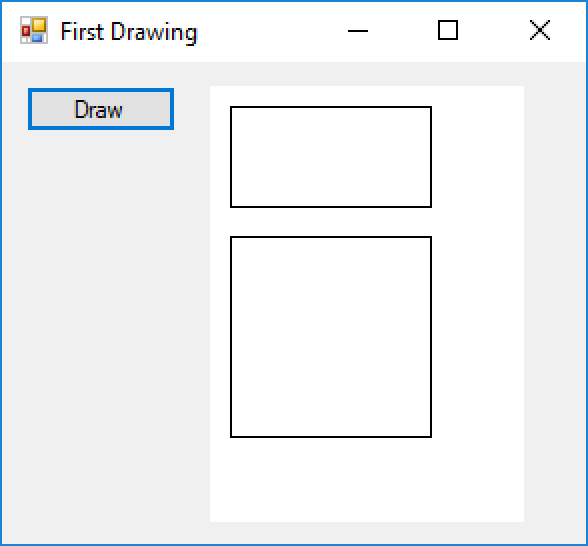
\includegraphics[width=8cm]{graphics_first}
			\caption{Screenshot of First Drawing program.}
			\label{fig:graphics_first}
		\end{figure}

		
	\section{Creating the program}
		To create this program, we use the IDE as explained in \Cref{ch:visual-studio}. Basically, the steps are:
		\begin{itemize}
			\item enter the VB IDE;
			\item create a new Windows Application project, named (for example) First Drawing.
		\end{itemize}
		Next, we need to place controls on the screen, so:
		\begin{itemize}
			\item Place a button and a picture box on the form. The exact positioning is not crucial – use the screenshot of Figure 3.1 as a guide. Click on the button, and change its \keyword{Text} property to \keyword{Draw}.
			\item Click on the picture box, and change its size property to \ui{150, 200}.
			\item Change the \keyword{BackColor} property of the picture box to a suitable colour. White is satisfactory. You can do this by opening up the drop-down list on the right of the \keyword{BackColor} property and choosing \ui{Custom}. Examples of colours appear; click on the white one.
			\item If you wish, you can alter the words used for the title of the form by clicking on the form, then setting its \keyword{Text} property to a meaningful title, e.g. \keyword{First Drawing}. In fact you can choose any title you like – it need not match the name of the project.
		\end{itemize}
		
		Here is a summary of the control settings:
		\begin{center}
			\begin{tabular}{lll}
				\toprule Control & Property & Setting\\ \midrule
				Button1	& Text&	Draw\\
				PictureBox1	& BackColor &	(Custom)  White \\
				PictureBox1 &	Size &	150, 200 \\
				Form1 &	Text &	First Drawing\\ \bottomrule
			\end{tabular}
		\end{center}

 
		The final stage in creating the program is to double-click on the button and insert the drawing instructions. All of the instructions go within the \keyword{Button1\_Click1} method, as shown in the above code.

		Run the program, then click on the 'Draw' button to see the two rectangles. If you have compilation errors, correct any typing mistakes, and try again. Typing errors are quite normal, so don't panic.
Now we will examine the detail of drawing shapes.

	\section{The graphics coordinate system}
		VB graphics are based on pixels. A pixel is a small dot on the screen which can be set to a particular colour. Each pixel is identified by a pair of numbers (its coordinates), starting from zero:
		\begin{itemize}
			\item the horizontal position, often referred to as x in mathematics, and also in the VB documentation. This value increases from left to right;
			\item the vertical position, often referred to as $y$ – this value increases downwards.
		\end{itemize}
		When we place a visual object on the screen, effectively we set its $x/y$ position. \Vref{fig:graphics_coordinates} shows a form of size 400 by 200, with a \keyword{PictureBox} placed at 200, 100. However, when drawing on the picture box, we regard \emph{its} top left corner as being the zero point of horizontal and vertical coordinates. In other words, we draw relative to the top left corner of the picture box, not relative to the top left corner of the form. This means that re-positioning the picture box has no effect on any drawing it contains. We use this system when we request VB to draw simple shapes.

		\begin{figure}[ht]
			\centering
			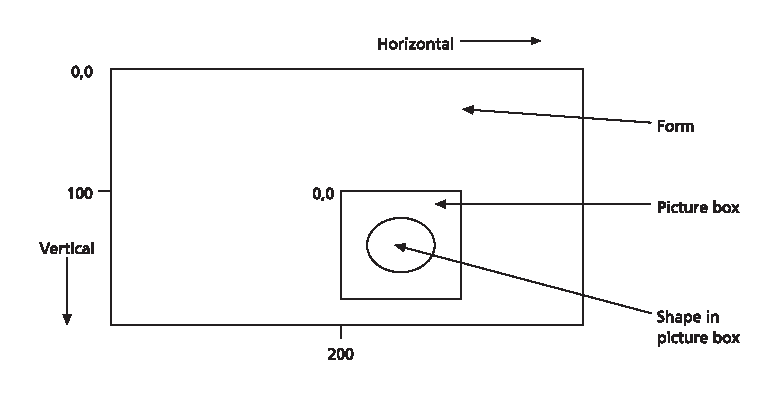
\includegraphics[width=\textwidth]{graphics_coordinates}
			\caption{Pixel coordinate system in VB.}
			\label{fig:graphics_coordinates}
		\end{figure}


		The size of the drawings depends on the quality of your screen, and on the graphics settings on your system. Higher-quality graphics have more (hence smaller) pixels, so your drawings will be smaller.

	\section{Explanation of the program}
		We will not explain every detail of each line here. There are some big ideas. But trust us that subsequent chapters will deal with them.

		Our drawing code is contained within one method, named Button1\_Click. There are two phases here: firstly we set up the drawing facilities, and then we actually draw. Here is the first part:
		\begin{lstlisting}[numbers=left]
Dim paper As Graphics
paper = PictureBox1.CreateGraphics()
Dim myPen As Pen = New Pen(Color.Black)
		\end{lstlisting}

		The good news is that the above lines will be the same for most of our drawing programs. We will provide a brief explanation of these lines, but it is not essential that you understand every detail at this stage.
		\begin{itemize}
			\item Line 1 is where we choose our name for the drawing area (we chose \keyword{paper}). The word \keyword{Dim} (short for 'dimension') allows us to choose a name for our object, and we must also choose its 'class' – i.e. its type. It is a \keyword{Graphics} item (rather than a \keyword{Button}, for example).
			\item In the second line, we link our drawing area to the picture box you placed on the form.
			\item In Line 3, we choose a name for our pen. The word \keyword{Pen} is already in use by VB – it is the name of a \emph{class} of item – so we went for \keyword{myPen}. At the same time, we set it to the colour black.
		\end{itemize}
		This completes the preparation for drawing. You should use these three identical lines in all the programs in this chapter. We are now ready to put some shapes on our picture box.

		To draw the shapes, we call (or invoke) VB's drawing methods. Here is the code:
		\begin{lstlisting}
paper.DrawRectangle(myPen, 10, 10, 100, 50)
paper.DrawRectangle(myPen, 10, 75, 100, 100)
		\end{lstlisting}

		The DrawRectangle method is one of the many methods provided by the VB system in a library. The statement shown is a call (also known as an invocation) of the method, asking it to carry out the task of displaying a rectangle. A method is so called because it is a method (or way) of doing something.

		When we make use of the DrawRectangle method, we need to supply it with a pen, and with values to fix its position and size. We need to get these in the correct order, which is:
		\begin{itemize}
			\item a \keyword{Pen} object;
			\item the horizontal value of the top left corner of the rectangle;
			\item the vertical value of the top left corner of the rectangle;
			\item the width of the rectangle;
			\item the height of the rectangle.
		\end{itemize}
		These items are known as arguments in VB. Other languages also use the term 'parameter'. Here, the arguments are inputs to the \keyword{DrawRectangle} method. Arguments must be enclosed in round brackets and separated by commas. This particular method requires five arguments, and they must be a \keyword{Pen} object, followed by four integers (whole numbers). If we attempt to use the wrong number of arguments, or the wrong type, we get an error message from the compiler. We need to ensure that:
		\begin{itemize}
			\item we supply the correct number of arguments;
			\item we supply the correct type of arguments;
			\item we arrange them in the right order.
		\end{itemize}
		Some methods do not require any arguments. In this case, we must still use the brackets, as in:
		\begin{lstlisting}
PictureBox1.CreateGraphics()
		\end{lstlisting}

		Here, we have been calling pre-written methods, but with VB's help we have written our own method. VB has named it \keyword{Button1\_Click}. We don't need to call it, because VB calls it for us when \keyword{Button1} is clicked. Its task is to call the \keyword{DrawRectangle} method twice. We shall cover the detail of writing our own methods in \Cref{ch:methods-arguments}.

	\section{Methods for drawing}
		As well as rectangles, VB provides us with facilities for drawing a range of shapes. Here, we have selected the simpler ones:
		\begin{itemize}
			\item lines;
			\item ellipses (i.e. ovals). These also include circles;
			\item filled rectangles and ellipses;
			\item images from files.
		\end{itemize}
		Additionally, we can change the colour of the pens we use for drawing, and use 'brushes' of a chosen colour to fill shapes.

		Here we list the arguments for each method, and provide an example program (Some Shapes) which uses them.
		\subsection*{\keyword{DrawRectangle}}
			\begin{itemize}
				\item a pen object;
				\item the horizontal value of the top left corner of the rectangle;
				\item the vertical value of the top left corner of the rectangle;
				\item the width of the rectangle;
				\item the height of the rectangle.
			\end{itemize}

		\subsection*{\keyword{DrawLine}}
			Note that this method does not use the concept of an enclosing rectangle. The arguments are:
			\begin{itemize}
				\item a pen object;
				\item the horizontal value of the start of the line;
				\item the vertical value of the start of the line;
				\item the horizontal value of the end of the line;
				\item the vertical value of the end of the line.
			\end{itemize}
		
		\subsection*{\keyword{DrawEllipse}}
			Imagine the ellipse (an oval) squeezed inside a rectangle. We provide:
			\begin{itemize}
				\item a pen object;
				\item the horizontal value of the top left corner of the rectangle;
				\item the vertical value of the top left corner of the rectangle;
				\item the width of the rectangle;
				\item the height of the rectangle.
			\end{itemize}
			To produce filled shapes we have:
		
		\subsection*{\keyword{FillRectangle}}
			Its coordinate arguments are mostly identical to those of the Draw equivalent. The main difference is that the first argument must be a Brush object rather than a pen. Brushes can use a range of colours and textures. Here we only show the simplest untextured 
version:

		\begin{lstlisting}
Dim myBrush As SolidBrush = New SolidBrush(Color.Black)
paper.FillRectangle(myBrush, 10, 10, 90, 90)
		\end{lstlisting}

		\subsection*{\keyword{FillEllipse}}
			This is used in a similar manner to DrawEllipse, but with a brush rather than a pen.
		
		\subsection*{\keyword{DrawImage}}
			This method is rather different, as it does not use preset shapes. Instead, it can be used to display images that have been stored in files. These images might have originated from a paint program, a scanner, camera or from the internet. To use \keyword{DrawImage}, we firstly create a \keyword{Bitmap} object by providing the name of a file containing an image. The bitmap is created with \keyword{Dim} in the same way as we created a \keyword{Pen} object earlier. We then use \keyword{DrawImage}, specifying the bitmap, the position of the image, and the size of its containing rectangle. The image is clipped (trimmed to fit) if it is too big for the rectangle. The Some Shapes program below shows how to create the bitmap object, which we chose to name as \keyword{pic}. Our image was taken from the Creative Commons website and saved as \keyword{imagedemo.jpeg}. We can also work with \keyword{gif} and \keyword{bmp} file types.
The 	order of arguments for \keyword{DrawImage} is:
		\begin{itemize}
			\item a bitmap object containing an image from a file.
			\item the horizontal value of the top left corner of the rectangle;
			\item the vertical value of the top left corner of the rectangle;
			\item the width of the rectangle;
			\item the height of the rectangle.
		\end{itemize}

	\section{Colours}
		It is possible to create as many pens and brushes as you wish, with their own colours. In VB, there are around 150 named colours. Below, we name the main colours, but also list some more obscure ones:
		\begin{center}
			\keyword{
			\begin{tabular}{lll}
				Black&	Violet&	Blue\\
				Indigo&	Green	&Yellow\\
				Orange&	Red	& Gray\\
				Purple&	White &	Firebrick\\
				LemonChiffon & Maroon &	OliveDrab
			\end{tabular}
			}
		\end{center}

		We use the colours when creating pens and brushes.
		
		Here is a program (called Some Shapes) which draws a variety of shapes. \Vref{fig:graphics_some_shapes} shows the resulting output.
		\begin{lstlisting}
Private Sub Button1_Click(
	sender As System.Object, 
	e As System.EventArgs) Handles Button1.Click
	Dim paper As Graphics
	paper = PictureBox1.CreateGraphics()
	Dim pic As New Bitmap("c:\mike\vbbook\imagedemo.jpeg")
	Dim myPen As Pen = New Pen(Color.Black)
	Dim fillBrush As SolidBrush = New SolidBrush(Color.Gray)
	paper.DrawRectangle(myPen, 10, 10, 100, 50)
	paper.DrawLine(myPen, 10, 10, 110, 60)
	paper.DrawRectangle(myPen, 10, 80, 100, 50)
	paper.DrawEllipse(myPen, 10, 80, 100, 50)
	paper.FillEllipse(fillBrush, 10, 150, 100, 50)
	paper.DrawRectangle(myPen, 130, 10, 150, 150)
	paper.DrawImage(pic, 130, 10, 150, 150)
End Sub
		\end{lstlisting}

		\begin{figure}[ht]
			\centering
			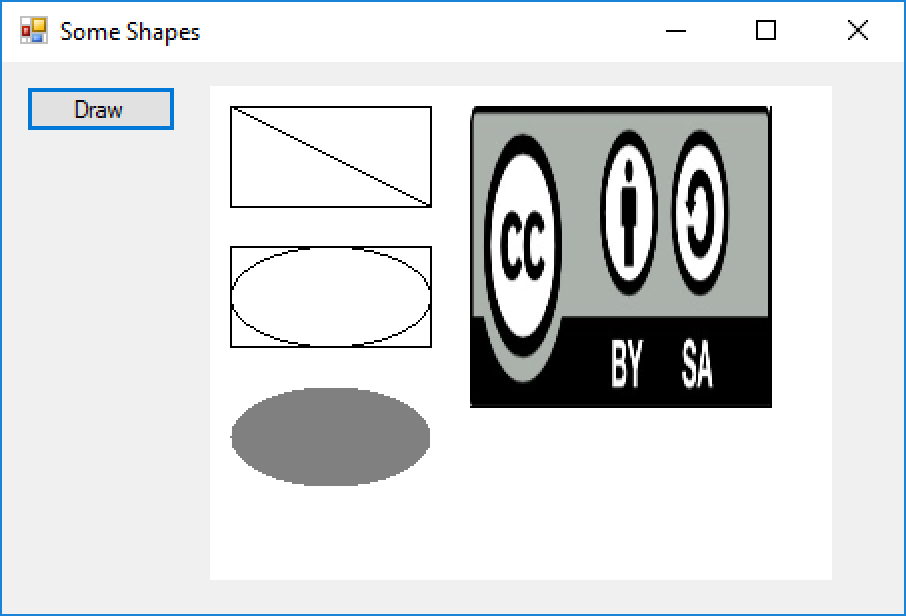
\includegraphics[width=8cm]{graphics_some_shapes}
			\caption{Screenshot of Some Shapes program.}
			\label{fig:graphics_some_shapes}
		\end{figure}


		Create the program in the same manner as the First Shapes one, but make the picture box larger: to \ui{300, 300}.

		\begin{stqb}
			\begin{STQ}
				\item	Write some VB instructions which produce a filled black circle of 50 pixels radius, 10 pixels in from the top left corner of a picture box.
			\end{STQ}
		\end{stqb}
	
	\section{The sequence concept and statements}
		When we have a number of instructions in a program, they are executed (obeyed, performed … ) in sequence, from the top of screen to the bottom (unless we specify otherwise using the concepts of selection and repetition covered in later chapters). However, you will not observe this because of the speed of the computer.
		
		In general, a VB program is composed of a series of 'statements'. There are many types of statements, such as a method call or an assignment. Some statements occupy a single line, but others (such as \keyword{If} and \keyword{While}, as we shall see) need to be written to spread over several lines.
		\begin{stqb}
			\begin{STQ}
				\item	Write and run a program which draws a large 'T' shape on the screen, with blue lines.
			\end{STQ}
		\end{stqb}

	\section{Adding meaning with comments}
		What does the following do?
		\begin{lstlisting}
paper.DrawLine(myPen, 20, 80, 70, 10)
paper.DrawLine(myPen, 70, 10, 120, 80)
paper.DrawLine(myPen, 20, 80, 120, 80)
		\end{lstlisting}

		The meianing is not instantly obvious, and you probably tried to figure it out with pencil and paper. The answer is that it draws a triangle with a horizontal base, but this is not apparent from the three statements. In VB, we can add comments (a kind of annotation) to the instructions, by preceding them by with ' (i.e. the single-quote key). For example, we might put:
		\begin{lstlisting}
' draw a triangle
paper.DrawLine(myPen, 20, 80, 70, 10)
paper.DrawLine(myPen, 70, 10, 120, 80)
paper.DrawLine(myPen, 20, 80, 120, 80)
		\end{lstlisting}

		A comment can contain anything – there are no rules. It is up to you to use them to convey meaning.
		
		Comments can also be placed at the end of a line, as in:
		\begin{lstlisting}
' draw a triangle
paper.DrawLine(myPen, 20, 80, 70, 10)
paper.DrawLine(myPen, 70, 10, 120, 80)
paper.DrawLine(myPen, 20, 80, 120, 80) ' draw base
		\end{lstlisting}

		Do not over-use comments. It is not normal to comment every line, as this often involves duplicating information. The following is a poor comment:

Dim aPen As Pen = New Pen(Color.Black) ' create a black pen
	
		Here, the statement says clearly what it does, without the need for a comment. Use comments to state the overall theme of a section of program, rather than restating the detail of each statement.
		
		\begin{stqb}
			\begin{STQ}
			\item	Provide a suitable comment for these lines:
		\begin{lstlisting}
paper.DrawLine(myPen, 0, 0, 100, 100)
paper.DrawLine(myPen, 100, 0, 100, 0)
\end{lstlisting}		
			\end{STQ}
		\end{stqb}

	\section{Programming principles}
		\begin{itemize}
			\item VB has a large collection of methods that we can call.
			\item The arguments we pass to graphics methods have the effect of controlling the shapes that are drawn.
		\end{itemize}

	\section{Programming pitfalls}
		Take care with punctuation and spelling. Commas and brackets must be exactly as in the examples.

	\section{Grammar spot}
		The order and type of arguments must be correct for each method.

	\section{New language elements}
		\begin{itemize}
			\item () to enclose arguments.
			\item The use of \keyword{Dim} to declare items.
			\item The use of New to create new objects.
			\item The use of the 'dot' notation to invoke methods of a class.
			\item ' to indicate comments.
		\end{itemize}

	\section{Summary}
		Statements are obeyed in sequence, top to bottom (unless we request otherwise).
		\begin{itemize}
			\item VB has a set of 'draw' methods which you can call up to display graphics.
			\item Graphics positioning is based on pixel coordinates.
			\item Argument values can be passed into methods.
		\end{itemize}


	\section{Exercises}
		In the following, we recommend that you do rough sketches and calculations prior to writing the program. You can use the same project for each question, using a picture box for drawing, and a button event to initiate the drawing.

		\begin{enumChapter}
			\item Write a program which draws a right-angled triangle. Choose an appropriate size.
			\item Write a program which draws an empty tic-tac-toe (noughts and crosses) board, made out of lines.
			\item Design a simple house, then write a program which draws it.
			\item	Here are some annual rainfall figures for the country of Xanadu, which we wish to display graphically:

			\keyword{
			\begin{tabular}{ll}
				1998  &  150 cm\\
				1999  &  175 cm\\
				2000  &  120 cm\\
				2001  &  130 cm
			\end{tabular}
			}
			\begin{itemize}
				\item Display the data as a series of horizontal lines.
				\item Instead of lines, use filled rectangles.
			\end{itemize}
		\item Write a program which displays an archery-style target with concentric circles of different colours. The purchase of a rubber sucker gun to fire at the screen is optional.
		\item Write a program which displays a simple face. The outline of the face, the eyes, ears, nose, and the mouth can be formed by ellipses.
		\end{enumChapter}


		\begin{stab}
			\begin{enumChapter}
				\item	We imagine that the circle is fitted inside a square whose sides are 100 pixels long:
					\begin{lstlisting}
Dim fillBrush As SolidBrush = New SolidBrush(Color.Black)
paper.FillEllipse(fillBrush, 10, 10, 100, 100)
					\end{lstlisting}
				\item 
					\begin{lstlisting}
paper.DrawLine(myPen, 20, 20, 120, 20)
paper.DrawLine(myPen, 80, 20, 80, 120)
					\end{lstlisting}
				\item The instructions draw a large 'X' on the picture box, so a suitable comment might be:
					\begin{lstlisting}
'draw an 'X' at top left
					\end{lstlisting}
			\end{enumChapter}
		\end{stab}
